   
\documentclass[11pt, answers]{exam}
\renewcommand{\baselinestretch}{1.05}
\usepackage{amsmath,amsthm,verbatim,amssymb,amsfonts,amscd, graphicx}
\usepackage{graphics}

\usepackage{tikz}
\usepackage{fancybox}

\usepackage{clrscode3e}

\topmargin0.0cm
\headheight0.0cm
\headsep0.0cm
\oddsidemargin0.0cm
\textheight23.0cm
\textwidth16.5cm
\footskip1.0cm
\theoremstyle{plain}
\newtheorem{theorem}{Theorem}
\newtheorem{corollary}{Corollary}
\newtheorem{lemma}{Lemma}
\newtheorem{proposition}{Proposition}
\newtheorem*{surfacecor}{Corollary 1}
\newtheorem{conjecture}{Conjecture}  
\theoremstyle{definition}
\newtheorem{definition}{Definition}

 \begin{document}
 


\title{CSC265: Assignment 1}
\author{Ruo yi Lin and Junjie Cheng}
\maketitle

\unframedsolutions

\begin{questions}

\question

\begin{parts}

\part Describe in detail a data structure implementing the Partial-Sums ADT. Draw an example with $n=8$, and values $a_1,\ldots,a_8$ of your choosing, but not $a_1=\ldots=a_8=0$. \\

\begin{solution}
The correct data structure is a full binary tree of height $k, B_k$. There are $2^k = n$ leaves in the lowest row of this tree. The $i$th leaf holds value $a_i$. The values of the parent nodes are defined recursively as the sum of their two children. An example is below with $a_1, \ldots, a_n = 1, 2, 3, 4, 5, 6, 7, 0$.
\\


\begin{center}
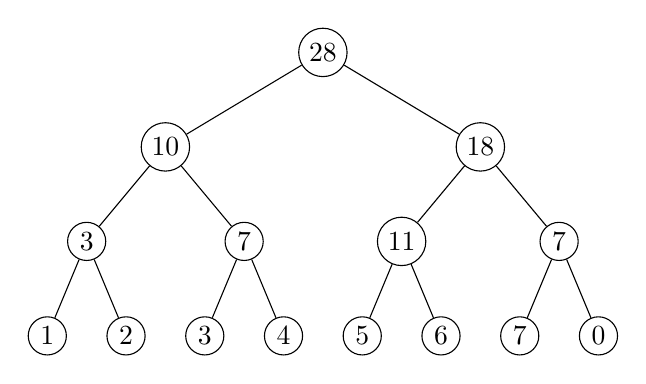
\begin{tikzpicture} 
[ 
level distance=12mm, 
every node/.style={circle, draw, inner sep=2pt},
level 1/.style={sibling distance=40mm}, 
level 2/.style={sibling distance=20mm}, 
level 3/.style={sibling distance=10mm}
]

\node {28} 
child {node {10} 
	child {node {3} 
		child {node {1}} 
		child {node {2}}
	}
	child {node {7} 
		child {node {3}} 
		child {node {4}}
	} 
}
child {node {18}
 	child {node {11} 
 		child {node {5}} 
 		child {node {6}}
 	}
 	child {node {7}
		child {node {7}}
		child {node {0}}
	}
};	 
\end{tikzpicture}
\end{center}

\end{solution}

\part Describe in clear and precise English how to implement the three operations $\proc{Init}$, $\proc{Add}(i,t)$, and $\proc{Sum}(i)$. Give pseudocode for $\proc{Add}(i,t)$, and $\proc{Sum}(i)$. For each operation argue why it computes the correct output, and show that it runs in the required worst-case running time.

\begin{itemize}
\item $\proc{Init}$ must run in time $\func{O}(n)$
\item $\proc{Add}(i,t)$ must run in time $\func{O}(\log(n))$
\item $\proc{Sum}(i)$ must run in time $\func{O}(\log(n))$
\end{itemize}

\begin{solution}\\

$\proc{Init}$:
Since $n = 2^k$, the binary tree required by the Partial-Sums ADT will always be full. Then the tree can be easily implemented as an array of size $2^{k+1} - 1$, with initial values all set to $0$. We assume that the first index of the array is $1$.

There is no need to construct pointers, since for a complete binary tree there are simple closed-form expressions for parent and child nodes. The functions are reproduced from CLRS Section 6.1.

Then $\proc{Init}$ runs in time $\func{O}(2^{k+1} - 1) = \func{O}(2(2^k)) = \func{O}(2n) = \func{O}(n)$.

\begin{codebox}
\Procname{$ \proc{Parent}(i)$}
\li 		\Return $\lfloor i/2 \rfloor$
\end{codebox}

\begin{codebox}
\Procname{$ \proc{Left-Child}(i)$}
\li 		\Return $2i$
\end{codebox}

\begin{codebox}
\Procname{$ \proc{Right-Child}(i)$}
\li 		\Return $2i + 1$
\end{codebox}

$\proc{Add}(i,t)$:
Add is simple to implement. The $i$th leaf of the tree is given by index $2^k + i$. We add $t$ to this leaf, and then add $t$ to each of $i$'s parents, grandparents, great-grandparents $\ldots$ until we reach the root.

\begin{codebox}
\Procname{$\proc{Add}(i,t)$}
\li $\func{node\_index} \gets 2^k + i$
\li \While $\func{node\_index} \neq 0$
\li \Do $\func{node\_index.value} \gets \func{node\_index.value} + t$
\li $\func{node\_index} = \proc{Parent}(\func{node\_index})$
\End
\end{codebox}

The resultant tree has an updated leaf and satisfies the sum property specified in $\proc{Init}$. This is because only the parents of the leaf specified by $i$ will have their values affected.

$\proc{Add}(i,t)$ runs in $\func{O}(\log(n))$. One iteration of the while loop is executed for each level of the tree, so the algorithm is proportional to the tree height. This in turn is proportional to the log of the number of nodes in the tree, which is proportional to the number of leaves. \\

We may reach the same conclusion by noticing that $\func{node\_index}$ is proportional to $n$ and that it is halved on each iteration when $\proc{Parent}$ is called.
\\

$\proc{Sum}(i)$:
We can implement $\proc{Sum}(i)$ by decomposing $i$ into its binary representation. Roughly speaking, the nodes at level $h$ of the tree hold values corresponding to sum of a group of $2^h$ elements of $(a_j)_{j=1}^{j=n}$. Then we can sum all of the elements $a_1, \ldots, a_i$ by travelling down the tree, and adding the value of at most one node from each level. We keep track of which powers of two we have already included, and which powers of two we still have left to include. When we have no more powers of two to include, the algorithm terminates, and the result is the sum $a_1, \ldots, a_i$.

In the pseudocode below, $i \func{div} c \gets \lfloor i \div c \rfloor$ and $i\mod c$ is the usual modulus function.

This algorithm is proportional to the height of the tree, and so it runs in $\func{O}(\log(n))$, as desired. 

\begin{codebox}
\Procname{$\proc{Sum}(i)$}
\li $\func{index} \gets 1$
\li $c \gets n$
\li $x \gets 0$
\li \While $i > 0$ \Do
\li		\If $i \func{div} c = 1$ \Do
\li 		$i \gets i - c$
\li			$x \gets x + \func{index.value}$
\li 		$\func{index} = 2\func{index} + 2$
			\End
\li		\Else \Do
\li			$\func{undex} = 2\func{index}$
			\End	
\li		$c \gets \lfloor c / 2 \rfloor$ 
\end{codebox}


\end{solution}




\part For each $n = 2^k$, and each setting of $a_1, \ldots, a_n$, give an input $i$, $1 \leq i \leq n$, such that your implementation of $\proc{Sum}(i)$ runs in time $\Omega(\log(n))$. Explain clearly and precisely why the running time is $\Omega(\log(n))$ on this input.


\begin{solution}

\end{solution}


\end{parts}


\question 

\begin{parts}

\part Give an algorithm for $\proc{Union}(H_1,H_2)$ running in worst-case time complexity $\func{O}(r_1 .d + r_2 .d)$ where $H_1$ and $H_2$ are $\proc{R-Heap}$ structures, $r_1$ is the root of $H_1$, $r_2$ is the root of $H_2$, and $H_1$ and $H_2$ are given to the algorithm by pointers to the roots $r_1$ and $r_2$, respectively.

$\proc{Union}(H_1,H_2)$ must return a pointer to the root of an $\proc{R-Heap}$ that contains the union of the elements of $H_1$ and $H_2$. Describe your algorithm in clear in precise English, and give pseudocode. Show that the running time of the algorithm is $\func{O}(r_1 .d + r_2 .d)$.

\begin{solution}

[Insert algorithm here.]

\begin{codebox}
\Procname{$\proc{Union}(H_1, H_2)$}

% base cases

\li \If $(r_1 == \func{NIL})$ \Then
\li 	\Return $r_2$
\li \ElseIf $(r_2 == \func{NIL})$ \Then
\li 	\Return $r_1$
\li \Else

% find the smaller key in the tree

\li	\If $(r_1.value	< r_2.value)$ \Then
\li		$\func{small} \gets r_1 $
\li		$\func{large} \gets r_2$
\li	\Else
\li		$\func{small} \gets r_2 $
\li		$\func{large} \gets r_1$
		\End
		
% merge left child of main tree 
		
\li	$\func{new\_child} \gets \proc{Union}(\func{small.left}, \func{large})$

% fixing parent

\li $\func{new\_child.parent} \gets \func{small}$

% recalculating d values
\li \If $\func{new\_child.left}$ and $\func{new\_child.right}$ \Then
\li $\func{new\_child.d} \gets {1+min\{new\_child.left.d, new\_child.right.d\}}$
\li \Else 
\li     ${new\_child.d = 1}$
        \End

% R-balance is preserved
\li \If $small.right == NIL$ or $small.right.d < small.left.d$   \Then
\li     small.left = small.right
\li     $small.right = \func{new\_child}$
\li \Else
\li     small.left = $\func{new\_child}$
        \End

\li 	\Return $\func{small}$
	\End
\end{codebox}

\textit{Partial Correctness}

Base case: (0, d) holds for all d, as does (d, 0)

One of the trees is empty, and the other satisfies the R-Heap property. The pointer to the root of the non-empty tree is returned. Vacuously, the condition holds.

Inductive case: want to show (d_1, d_2).
assume (d_1 -1, d_2)

Assume that the union operation 

\textit{Proof of Termination.}

Loop invariant: the algorithm runs in the time complexity ...

base case 


\end{solution}

\part 

\begin{solution}

\end{solution}

\part Recall that the height of a tree $T$ with root $r$ equals the number of edges in the longest path from $r$ to a leaf of $T$. What is the largest possible height of an $\proc{R-Heap}$ with $n$ nodes?

\begin{solution}
The largest possible height is $n-1$.

Note that in general the largest possible height for a binary tree of $n$ nodes is given by $n-1$: each node in the tree has exactly one child. To construct such a tree which satisfies the $\proc{R-Heap}$ properties, 


\end{solution}


\end{parts}
\end{questions}

 
\end{document}